% Deffinitions
\documentclass[12pt, a4paper, oneside]{article}

\usepackage{fancyhdr, ifpdf}
\usepackage[ansinew]{inputenc}
\usepackage{listings}
\usepackage[hyphens]{url}
\usepackage{subfig}
\usepackage{graphicx}
\usepackage{float}
\usepackage{dirtree}
\usepackage{xcolor}
\usepackage{longtable}
\usepackage{tabularx}


\definecolor{clr-background}{RGB}{255,255,255}
\definecolor{clr-text}{RGB}{0,0,0}
\definecolor{clr-string}{RGB}{163,21,21}
\definecolor{clr-namespace}{RGB}{0,0,0}
\definecolor{clr-keyword}{RGB}{0,0,255}
\definecolor{clr-type}{RGB}{43,145,175}
\definecolor{clr-variable}{RGB}{0,0,0}
\definecolor{clr-constant}{RGB}{111,0,138}
\definecolor{clr-comment}{RGB}{0,128,0}

\lstdefinestyle{VSC}{
	backgroundcolor=\color{clr-background},
	basicstyle=\color{clr-text},
	stringstyle=\color{clr-string},
	identifierstyle=\color{clr-variable},
	commentstyle=\color{clr-comment},
	keywordstyle=\color{clr-type},
	keywordstyle={[2]\color{clr-constant}},
	tabsize=4,
	numbers=left,
	numbersep=5pt
}

\lstloadlanguages{[Visual]C++}
\lstset{style=VSC}
                
\PassOptionsToPackage{hyphens}{url}\usepackage{hyperref}


\pagestyle{fancyplain}

% Document Entry
\begin{document}

% Title Sheet
\author{ Ludwig F{\"u}chsl }
\title{DualSense Windows API \protect\\ Version 0.1}
\date{\today}
\maketitle

% Content
\pagenumbering{arabic}
\tableofcontents

% Include
\section{Important information}
\subsection{Trademarks and affiliation}
"PlayStation", "PlayStation Family Mark", "PS5 logo", "PS5", "DualSense" and "DUALSHOCK" are registered trademarks or trademarks of Sony Interactive Entertainment Inc. "SONY" is a registered trademark of Sony Corporation.

\textbf{The Author is not affiliated in any kind with Sony Interactive Entertainment Inc.!} \\
Using this library may void your / your clients / your users / your customers controllers warranty! You as the redistributor of the precompiled or self compiled library have to make sure the controller will not be damaged by the functionality you use or at least point out the possible risk to your users / clients / customer!\\
Probably no damage or failure at all. This statement is just for my own safety!

\subsection{Sources}
This work is derivative from others work. Special thanks goes to:
\begin{itemize}
	\item GitHub user dogtopus: \\ \url{https://gist.github.com/dogtopus/894da226d73afb3bdd195df41b3a26aa}.
	\item Reddit user ginkgobitter: \url{https://www.reddit.com/r/gamedev/comments/jumvi5/dualsense_haptics_leds_and_more_hid_output_report/}
	\item GitHub user Ryochan7: \url{https://github.com/Ryochan7/DS4Windows/tree/dualsense-integration} \\ Copyright (c) 2019 Travis Nickles - MIT License: \url{https://github.com/Ryochan7/DS4Windows/blob/jay/LICENSE.txt} 
	\item And the amazing community at DS4Windows \url{https://github.com/Ryochan7/DS4Windows/issues/1545}
	
\end{itemize}
\newpage

\subsection{License}
\textbf{MIT License}\\

Copyright (c) 2020 Ludwig F�chsl\\

Permission is hereby granted, free of charge, to any person obtaining a copy of this software and associated documentation files (the "Software"), to deal in the Software without restriction, including without limitation the rights to use, copy, modify, merge, publish, distribute, sublicense, and/or sell copies of the Software, and to permit persons to whom the Software is furnished to do so, subject to the following conditions:\\

The above copyright notice and this permission notice shall be included in all copies or substantial portions of the Software.\\

THE SOFTWARE IS PROVIDED "AS IS", WITHOUT WARRANTY OF ANY KIND, EXPRESS OR IMPLIED, INCLUDING BUT NOT LIMITED TO THE WARRANTIES OF MERCHANTABILITY, FITNESS FOR A PARTICULAR PURPOSE AND NONINFRINGEMENT. IN NO EVENT SHALL THE AUTHORS OR COPYRIGHT HOLDERS BE LIABLE FOR ANY CLAIM, DAMAGES OR OTHER LIABILITY, WHETHER IN AN ACTION OF CONTRACT, TORT OR OTHERWISE, ARISING FROM, OUT OF OR IN CONNECTION WITH THE SOFTWARE OR THE USE OR OTHER DEALINGS IN THE SOFTWARE.

\newpage
\section{Introduction}
Welcome to the DualSense on Windows API documentation. This API will help you integrating the Sony PS5 DualSense controller into your application or game for Windows. This document will guide you through the complete flow of integration. Starting with learning the DualSense Features up to deeply understanding every feature of this api.\\
The documentation is structured as follows:
\begin{itemize}
	\item Descriptions of the DualSense's features
	\item installation and self compiling
	\item getting started guide
	\item api references
\end{itemize}

We recommend starting with reading through all features as far as you are not familiar with the DualSense controllers feature. Continuing with the installation and getting started guide to get your own demo application up and running. Then you can use the API references to integrate the api into your application.

\newpage
\section{Features}
In the following section the features of the DualSense controller will be explained.

\subsection{Overview}
\begin{itemize}
	\item \textbf{Connectivity} The DualSense controller can be used via Bluetooth or USB (USB C).
	\item \textbf{Integrated battery} Featuring an integrated battery the DualSense controller is best used via Bluetooth. The controller can be charged via USB type-C.
\end{itemize}

\begin{figure}[H]
    \centering
    \subfloat[\centering Front View]{{
\includegraphics[width=5cm]{frontView} }}
    \qquad
    \subfloat[\centering Rear View]{{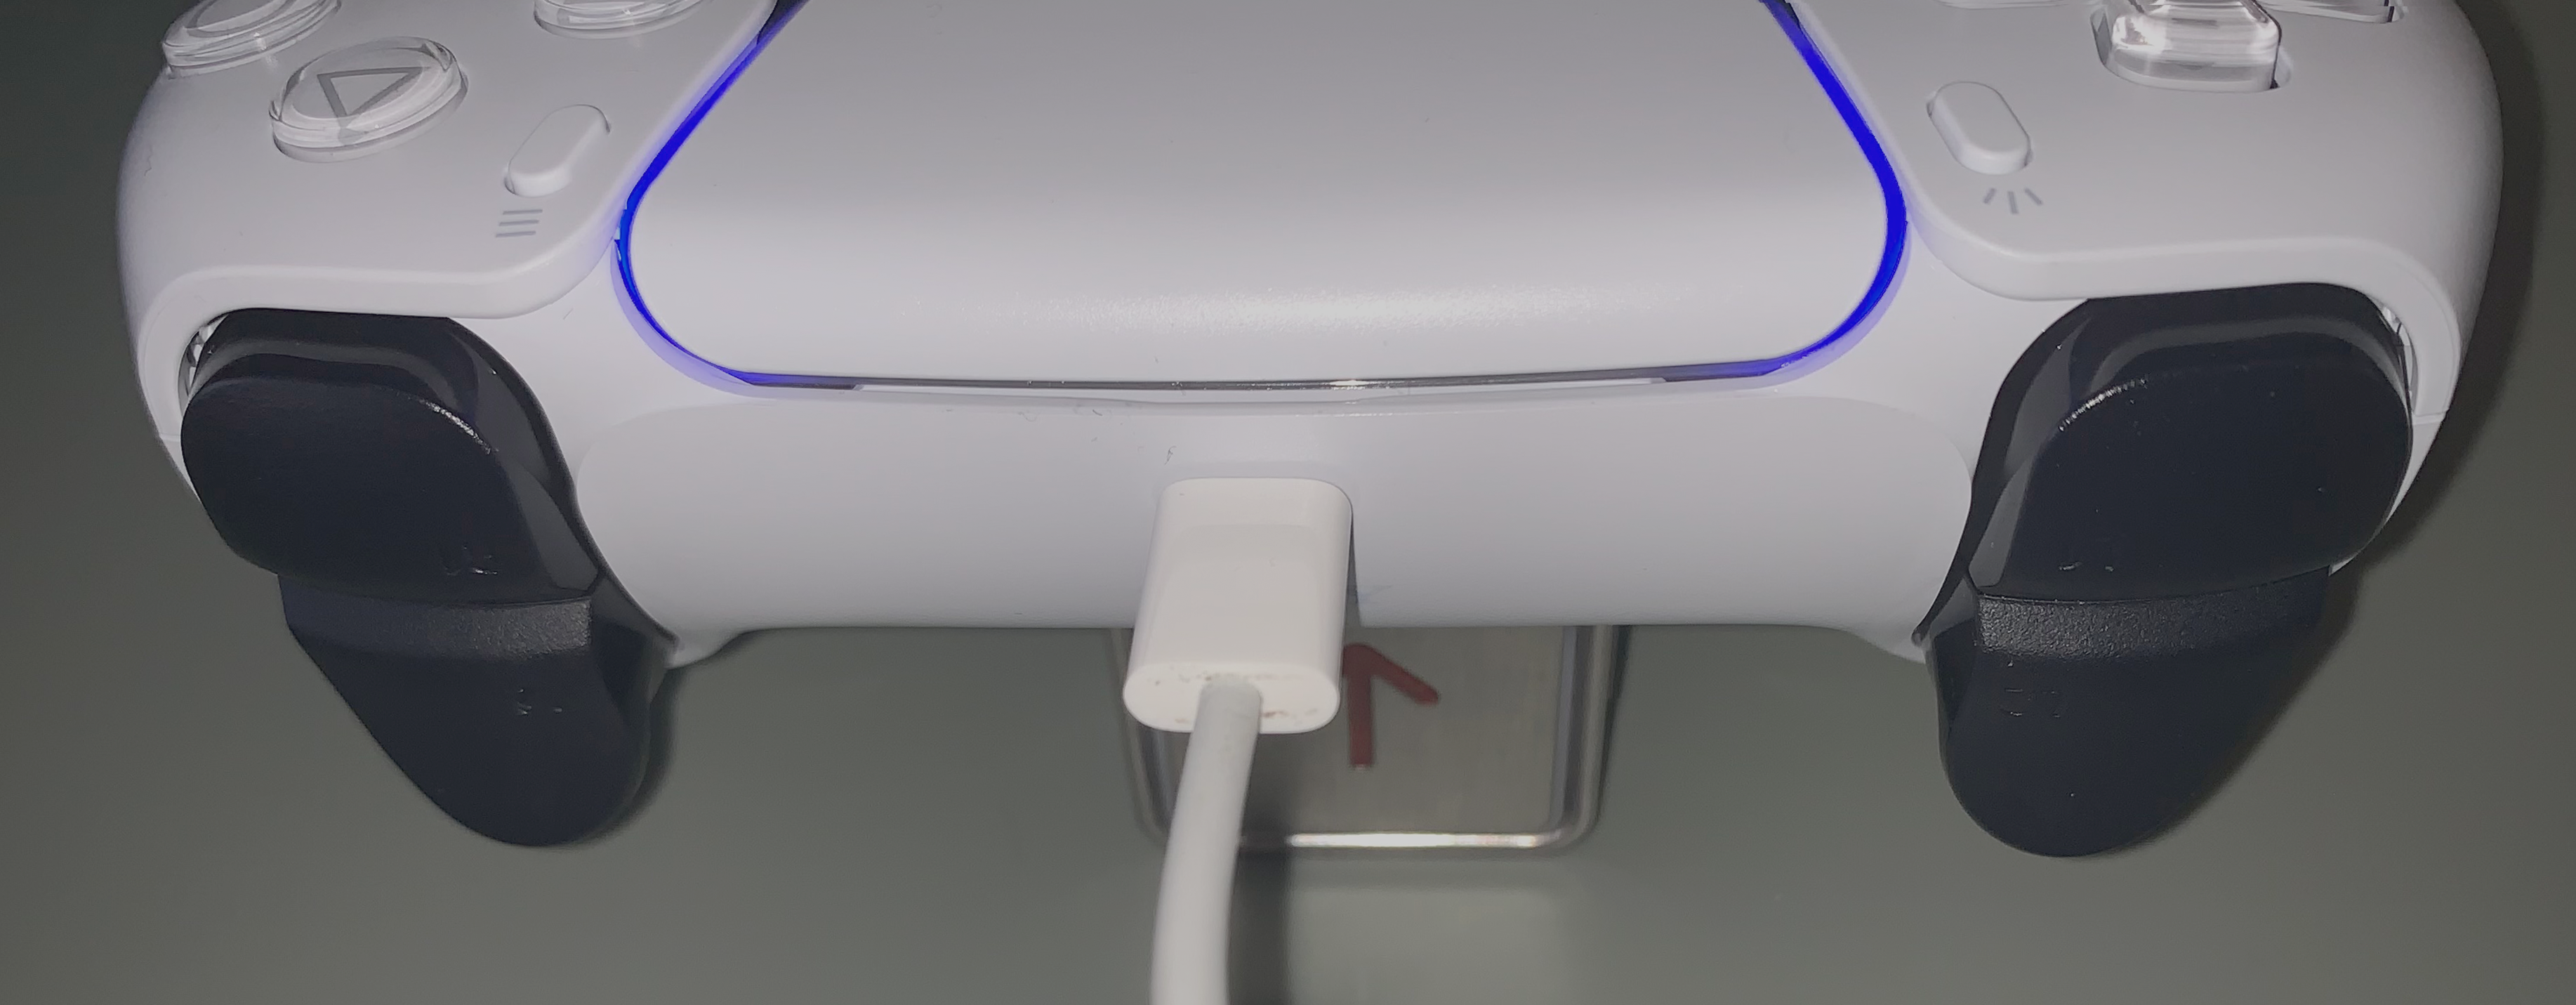
\includegraphics[width=5cm]{rearView} }}
    \caption{The DualSense controller}
\end{figure}

The DualSense controller features the following peripherals:
\begin{itemize}
	\item Two XY-Axis analog sticks with integrated push button.
	\item Two adaptive triggers (are able to provide feedback).
	\item Two shoulder buttons.
	\item DPad with the ability to press two neighbor buttons simultaneously.
	\item The default Square, Cross, Circle and Triangle PlayStation buttons.
	\item Dual-touch touchpad with integrated push button, surrounded with five player indication LEDs on the bottom and RGB-LED lightbar on the sides.
	\item Menu, share, microphone mute and PlayStation button.
	\item 3-Axis Accelerometer and Gyroscope.
	\item Two rumble motors (Hard and Soft one). Can alternatively used as haptic feedback (not supported yet).
	\item Integrated speaker and microphone.
	\item Stereo audio jack.	
\end{itemize}

\subsection{Feature List}

\paragraph{Analog sticks}
Each analog stick has two axis with 8-Bit precision each. The analog sticks will automatically return to their center position if released. They are mapped to the range $-128$ to $127$ where $0$ means center, $-128$ means left/bottom on X/Y-Axis and $127$ means right/top on X/Y-Axis. Using the analog values requires the correction of the dead zones, because a released stick will most likely not have the value $R_{xy}(0; 0)$ it will be a bit off. Same goes for the extreme values witch will also be off and not be exactly $T_{xy}(0; 127)$, $L_{xy}(-128; 0)$, etc..
\begin{figure}[H]
    \centering
    \subfloat{{\includegraphics[width=8cm]{frontView_sticks} }}
    \caption{Analog sticks}
\end{figure}

\paragraph{Adaptive trigger}
The DualSense controller feature two 8-Bit analog triggers. It is possible to read the trigger values as 8-Bit continuous values or alternatively as binary button input. Aside of the normal trigger operation the adaptive triggers can be configured to simulate various force feedback effects. It is possible for example to simulate a gun trigger.
\begin{figure}[H]
    \centering
    \subfloat{{\includegraphics[width=8cm]{rearView_trigger} }}
    \caption{Adaptive triggers}
\end{figure}

\paragraph{Bumpers}
The two L/R Bumpers located over the adaptive triggers can be read as normal button inputs.
\begin{figure}[H]
    \centering
    \subfloat{{\includegraphics[width=8cm]{rearView_bumpers} }}
    \caption{L/R Bumpers}
\end{figure}

\paragraph{DPAD and PS Buttons}
The DualSense controller feature a DPAD and the default well know PlayStation Square, Cross, Circle and Triangle buttons. The DPAD is capable of registering two simultaneously pressed buttons, however the two buttons must be neighbors. The PS-Buttons are being registered as four individual binary values.
\begin{figure}[H]
    \centering
    \subfloat{{\includegraphics[width=8cm]{frontView_mainbtn} }}
    \caption{DPAD and PS-Buttons}
\end{figure}

\paragraph{Other Buttons}
The DualSense controller feature several more buttons. Thees are:
\begin{itemize}
	\item \textbf{Menu button} Should be used to open the in-game menu.
	\item \textbf{Share button} Should be used to open the in-game photo mode.
	\item \textbf{PlayStation button} Can be used to open a in-game overlay (Look at the know issues to get an additional use case of this button).
	\item \textbf{Mic button} Should be used to mute the microphone.
\end{itemize}
All the listed buttons are readable through individual binary values.
\begin{figure}[H]
    \centering
    \subfloat{{\includegraphics[width=8cm]{frontView_other} }}
    \caption{Left to right, top to bottom: Share, Menu, PlayStation and Mic Button}
\end{figure}

\paragraph{Touch Pad}
The touch-pad and the surrounding lightbar are featuring several functions:
\begin{itemize}
	\item \textbf{Dual finger touch} The touch-pad itself is able to track two fingers simultaneously.
	\item \textbf{Integrated push button} The touch-pad integrates as momentary push button operated by pushing the pad down.
	\item \textbf{Lightbar} The left and right surrounding is able to light up in full 8-Bit RGB colors. The lib is providing several helpers to convert other color formats to the 8-Bit RGB UCHAR formate.
	\item \textbf{Player indication LEDs} On the bottom of the touch-pad are five player indication LEDs located. Thees LEDs are group in one left, three middle and one right led. The brightness of the LEDs is controllable and the LEDs are able to fade in.
\end{itemize}
When using the touch-pad make sure to implement hysteresis, dead zones and tolerances. It may also helpful to accumulate the values over multiple frame to get a more stable result but this will also increase latency. 
\begin{figure}[H]
    \centering
    \subfloat{{\includegraphics[width=8cm]{frontView_touch} }}
    \caption{Touch Pad}
\end{figure}

\paragraph{Accelerometer and Gyroscope}
The DualSense controller is able to measure its acceleration (By moving the controller around) and to track its rotation. Measurements are done with 16-Bit precision in all three XYZ-Axis. Make sure to implement hysteresis, dead zones and tolerances. It may also helpful to accumulate the values over multiple frame to get a more stable result but this will also increase latency.
\begin{itemize}
	\item \textbf{Accelerometer} Measures the acceleration.
	\item \textbf{Gyroscope} Measures the controllers rotation. Currently you have to implement calibration in your own codebase. 
\end{itemize}

\paragraph{Rumble motors / Haptic feedback}
The DualSense feature two Haptic feedback devices. Thees device work similar like normal speaker, but they are not good in producing tones, they are good in producing vibration. It is possible to send an audio signal directly to those haptic speakers (However currently not supported by this API).\\
The controller supports simulating the normal soft and hard rumble motors using the haptic speakers. When using this mode both motors can be controlled with the usual 8-Bit values. The left rumble feels hard, the right one soft.

\paragraph{Integrated speaker and microphone}
Featuring two microphones and one mono speaker, the DualSense is able to produce and pickup audio. This features will be supported in the future. However it is possible to address thees devices with the default WASAPI independently. 

\paragraph{Stereo audio jack}
Directly under the little microphone icon is a stereo headphone audio jack. It is possible to retrieve the connection status of this jack. However just like the speaker it is currently not supported to produce audio through the API.

\newpage
\section{Installation}
Bla install

\subsection{Prebuild installation}
prebuild

\subsection{Self build installation}
own build

\newpage
\section{Quick start}
Quick start

\newpage
\section{API Reference}
\subsection{Preprocessor constants}

\newcolumntype{b}{>{\hsize=.66\hsize}X}
\newcolumntype{s}{>{\hsize=.33\hsize}X}

\newcommand{\tblx}[2]{
	\noindent
	\begin{tabularx}{\textwidth} { | >{\raggedright\arraybackslash}X |  }
		\hline
		\texttt{#1} \\
		\hline
		#2 \\
		\hline
	\end{tabularx}
	\mbox{}\\

}

\newcommand{\tbly}[3]{
	\noindent
	\begin{tabularx}{\textwidth}{|s|b|}
		\midrule % hline
			#1 & \texttt{#2} \\
		\midrule % hline
			\multicolumn{2}{|l|}{\begin{minipage}{0.9\linewidth} \noindent #3 \end{minipage}} \\ % \rule{0pt}{2ex} \rule{0pt}{2ex} 
		\midrule % hline
	\end{tabularx}
	\mbox{}
}

\paragraph{Error codes}
\mbox{}\\

% DS5W_OK
\tblx{DS5W\_OK}{The operation completed without an error}

% DS5W_E_UNKNOWN
\tblx{DS5W\_E\_UNKNOWN}{An unknown error occurred}

% DS5W_E_INSUFFICIENT_BUFFER
\tblx{DS5W\_E\_INSUFFICIENT\_BUFFER}{The user supplied buffer is to small }

% DS5W_E_EXTERNAL_WINAPI
\tblx{DS5W\_E\_EXTERNAL\_WINAPI}{An unsuspected Windows sided error occurred}

% DS5W_E_INVALID_ARGS
\tblx{DS5W\_E\_INVALID\_ARGS}{The user supplied arguments are invalid}

% DS5W_E_CURRENTLY_NOT_SUPPORTED
\tblx{DS5W\_E\_CURRENTLY\_NOT\_SUPPORTED}{This feature is currently not supported}

% DS5W_E_DEVICE_REMOVED
\tblx{DS5W\_E\_DEVICE\_REMOVED}{The device was removed unexpectedly}

% DS5W_E_BT_COM
\tblx{DS5W\_E\_BT\_COM}{Bluetooth communication error}



\paragraph{Error helpers}
\mbox{}\\

% DS5W_SUCCESS(expr)
\tblx{DS5W\_SUCCESS(expr)}{Check if the user supplied expression is an error success code}

% DS5W_FAILED(expr)
\tblx{DS5W\_FAILED(expr)}{Check if the user supplied expression is an error code}



\paragraph{I/O State helpers}
\mbox{}\\

% DS5W_ISTATE_BTX_SQUARE / CROSS / CIRCLE / TRIANGLE
\tblx{DS5W\_ISTATE\_BTX\_SQUARE}{PlayStation Square button}
\tblx{DS5W\_ISTATE\_BTX\_CROSS}{PlayStation Cross button}
\tblx{DS5W\_ISTATE\_BTX\_CIRCLE}{PlayStation Circle button}
\tblx{DS5W\_ISTATE\_BTX\_TRIANGLE}{PlayStation Triangle button}

% DPAD
\tblx{DS5W\_ISTATE\_DPAD\_LEFT}{D-Pad left}
\tblx{DS5W\_ISTATE\_DPAD\_DOWN}{D-Pad down}
\tblx{DS5W\_ISTATE\_DPAD\_RIGHT}{D-Pad right}
\tblx{DS5W\_ISTATE\_DPAD\_UP}{D-Pad up}

% Button A
\tblx{DS5W\_ISTATE\_BTN\_A\_LEFT\_BUMPER}{Left bumper button}
\tblx{DS5W\_ISTATE\_BTN\_A\_RIGHT\_BUMPER}{Right bumper button}
\tblx{DS5W\_ISTATE\_BTN\_A\_LEFT\_TRIGGER}{Left trigger binary input}
\tblx{DS5W\_ISTATE\_BTN\_A\_RIGHT\_TRIGGER}{Right trigger binary input}
\tblx{DS5W\_ISTATE\_BTN\_A\_SELECT}{Select / Share button}
\tblx{DS5W\_ISTATE\_BTN\_A\_MENU}{Menu Button}
\tblx{DS5W\_ISTATE\_BTN\_A\_LEFT\_STICK}{Left stick push button}
\tblx{DS5W\_ISTATE\_BTN\_A\_RIGHT\_STICK}{Right stick push button}

% Button B
\tblx{DS5W\_ISTATE\_BTN\_B\_PLAYSTATION\_LOGO}{PlayStation logo button}
\tblx{DS5W\_ISTATE\_BTN\_B\_PAD\_BUTTON}{The touch-pads integrated button}
\tblx{DS5W\_ISTATE\_BTN\_B\_MIC\_BUTTON}{Microphone mute button}

% Outstate
\tblx{DS5W\_OSTATE\_PLAYER\_LED\_LEFT}{Left player indicator LED bit-mask}
\tblx{DS5W\_OSTATE\_PLAYER\_LED\_MIDDLE\_LEFT}{Left middle player indicator LED bit-mask}
\tblx{DS5W\_OSTATE\_PLAYER\_LED\_MIDDLE}{Middle player indicator LED bit-mask}
\tblx{DS5W\_OSTATE\_PLAYER\_LED\_MIDDLE\_RIGHT}{Right middle player indicator LED bit-mask}
\tblx{DS5W\_OSTATE\_PLAYER\_LED\_RIGHT}{Right player indicator LED bit-mask}

\subsection{Types}
\paragraph{DeviceEnumInfo} This struct contains all internal data required for the controller enumeration. You should not read or write any of the internal data directly. The struct can be freely user allocated with random data. It will be initialized by the corresponding function call, don't use it before it got initialized by the corresponding function.

\paragraph{DeviceContext} This struct contains all internal data for reading and writing to the controller. You should not read or write any of the internal data directly. The struct can be freely user allocated with random data. It will be initialized by the corresponding function call, don't use it before it got initialized by the corresponding function. It is very important to free this data with the corresponding function before the application exits or memory is reused. 

\label{APIRef_Types_analstick}
\paragraph{AnalogStick} This struct represent the XY position of one analog stick. Make sure to implement dead zones by yourself! \\

\tbly{int8\_t}{x}{X Position (left to right) of the analog stick.} \\

\tbly{int8\_t}{y}{Y Position (top to bottom) of the analog stick.} \\

\label{APIRef_Types_vec3}
\paragraph{Vector3, Vec3} Represents a three component 16-Bit vector \\

\tbly{int16\_t}{x}{X Component} \\

\tbly{int16\_t}{y}{Y Component} \\

\tbly{int16\_t}{z}{Z Component} \\

\label{APIRef_Types_color}
\paragraph{Color} RGB 8-Bit color components. The library also provides several conversion functions to turn several color formats into 8-Bit RGB values.\\

\tbly{uint8\_t}{r}{R - Red color channel}\\

\tbly{uint8\_t}{g}{G - Green color channel}\\

\tbly{uint8\_t}{b}{B - Blue color channel}\\

\label{APIRef_Types_touch}
\paragraph{Touch} This struct contains information about a single fingers touch position. \\

\tbly{int8\_t}{x}{X Position of the finger (left to right).} \\

\tbly{int8\_t}{y}{Y Position of the finger (top to bottom).} \\

\label{APIRef_Types_micled}
\paragraph{MicLed} Enum class representation the state of the microphone LED. \\

\tblx{OFF}{Microphone LED is completely off}
\tblx{ON}{Microphone LED is on}
\tblx{PULSE}{Microphone LED is pulsing}


\label{APIRef_Types_tfxt}
\paragraph{TriggerEffectType} Enum class: feedback / effect type of the adaptive trigger.\\

\tblx{NoResitance}{Adaptive trigger is disabled. Will provide no resistance.}
\tblx{ContinuousResitance}{Adaptive trigger will provide a continuous resistance from a specific starting point.}
\tblx{SectionResitance}{Adaptive trigger will provide a force fixed resistance on a defined section.}
\tblx{EffectEx}{Adaptive trigger will execute an extended effect.}
\tblx{Calibrate}{Adaptive trigger will enter an fixed function calibration program. Still experimental use only!}

\label{APIRef_Types_trigfx}
\paragraph{TriggerEffect}
This struct represents an adaptive trigger effect. The first param is the type. The other is a union over structs for each type.\\

\tbly{\hyperref[APIRef_Types_tfxt]{TriggerEffectType}}{effectType}{Type of the effect. Chose next data according to this parameter.}\\

\noindent
When \texttt{effectType} == \texttt{NoResitance} no parameter needs to be set!\\
When \texttt{effectType} == \texttt{Calibrate} no parameter needs to be set!\\
When \texttt{effectType} == \texttt{ContinuousResitance}:\\

\tbly{uint8\_t}{Continuous.startPosition}{Start position of the continuous force.}\\

\tbly{uint8\_t}{Continuous.endPosition}{Force applied.}\\

\noindent
When \texttt{effectType} == \texttt{SectionResitance}:\\

\tbly{uint8\_t}{Section.startPosition}{Start of force increased area.}\\

\tbly{uint8\_t}{Section.force}{End of force increased area.}\\

\noindent
When \texttt{effectType} == \texttt{EffectEx}:\\

\tbly{uint8\_t}{EffectEx.startPosition}{Start positions of the effect.}\\

\tbly{bool}{EffectEx.keepEffect}{Indicates weather the effect should keep playing (vibration) when the trigger is fully pressed.}\\

\tbly{uint8\_t}{EffectEx.beginForce}{Force for the section with trigger value >= 128.}\\

\tbly{uint8\_t}{EffectEx.middleForce}{Force for the section with trigger value <= 128.}\\

\tbly{uint8\_t}{EffectEx.endForce}{Force applied when the trigger is fully pressed / would go beyond 255.}\\

\tbly{uint8\_t}{EffectEx.frequency}{Frequency with witch the effect is executed. More a scalar value to scale between two fixed frequency than an read frequency parameter,}\\


\label{APIRef_Types_ledbr}
\paragraph{LedBrightness} Enum class representation the brightness of the player indication LEDs.\\

\tblx{LOW}{Low brightness player indication LEDs}
\tblx{MEDIUM}{Medium brightness player indication LEDs}
\tblx{HIGH}{High brightness player indication LEDs}

\label{APIRef_Types_pleds}
\paragraph{PlayerLeds} Struct defining the player LDEs state.\\

\tbly{Bitmask / uint8\_t}{bitmask}{Bitmask of the enabled player indication LEDs. Or together all enabled LEDs by using the \texttt{DS5W\_OSTATE\_PLAYER\_LED\_XXXXX} macros.}\\

\tbly{bool}{playerLedFade}{Indicates weather the player LEDs should fade in when enabled.}\\

\tbly{\hyperref[APIRef_Types_ledbr]{LedBrightness}}{brightness}{Brightness of the player LEDs}\\


\paragraph{DS5InputState} 
This struct represents the input state of a DualSense controller. It is used to read all input data.\\

\tbly{\hyperref[APIRef_Types_analstick]{AnalogStick}}{leftStick}{Represents the position of the left analog stick.}\\

\tbly{\hyperref[APIRef_Types_analstick]{AnalogStick}}{rightStick}{Represents the position of the right analog stick.}\\

\tbly{uint8\_t}{leftTrigger}{8-Bit position of the left trigger. No dead zones required!}\\

\tbly{uint8\_t}{rightTrigger}{8-Bit position of the right trigger. No dead zones required!}\\

\tbly{Bitmask / uint8\_t}{buttonsAndDpad}{Bitmask of the PlayStation button and the DPAD. Check the active state with the \texttt{DS5W\_ISTATE\_BTX\_XXXXX} and \texttt{DS5W\_ISTATE\_DPAD\_XXXXX} macros.}\\

\tbly{Bitmask / uint8\_t}{buttonsA}{Bitmask of the controllers buttons (Set A). Check the active state with the \texttt{DS5W\_ISTATE\_BTN\_A\_XXXXX} macros.}\\

\tbly{Bitmask / uint8\_t}{buttonsB}{Bitmask of the controllers buttons (Set B). Check the active state with the \texttt{DS5W\_ISTATE\_BTN\_B\_XXXXX} macros.}\\

\tbly{\hyperref[APIRef_Types_vec3]{Vector3}}{accelerometer}{Acceleration vector.}\\

\tbly{\hyperref[APIRef_Types_vec3]{Vector3}}{gyroscope}{Orientation vector.}\\

\tbly{\hyperref[APIRef_Types_touch]{Touch}}{touchPoint1}{First touch point.}\\

\tbly{\hyperref[APIRef_Types_touch]{Touch}}{touchPoint2}{Second touch point.}\\

\tbly{bool}{headPhoneConnected}{Indicates weather a plug is present in the headphone jack. Will also trigger on an extension cord with no headphone connected!}\\

\tbly{uint8\_t}{leftTriggerFeedback}{Indicates the pressing force when the left adaptive trigger is active.}\\

\tbly{uint8\_t}{rightTriggerFeedback}{Indicates the pressing force when the right adaptive trigger is active.}\\


\paragraph{DS5OutputState}
This struct represents the output state of a DualSense controller. It is used to set all output data. \\

\tbly{uint8\_t}{leftRumble}{Force of the left (hard) rumble motor.}\\

\tbly{uint8\_t}{rightRumble}{Force of the right (soft) rumble motor.}\\

\tbly{\hyperref[APIRef_Types_micled]{MicLed}}{microphoneLed2}{State of the microphone LED.}\\

\tbly{bool}{disableLeds}{When active the lightbar will be set to the default PS5 blue.}\\

\tbly{\hyperref[APIRef_Types_pleds]{PlayerLeds}}{playerLeds}{State of the player LEDs.}\\

\tbly{\hyperref[APIRef_Types_color]{Color}}{lightbar}{RGB Color of the lightbar. No affect when \texttt{disableLeds} is \texttt{true}}\\

\tbly{\hyperref[APIRef_Types_trigfx]{TriggerEffect}}{leftTriggerEffect}{Effect of the left adaptive trigger.}\\

\tbly{\hyperref[APIRef_Types_trigfx]{TriggerEffect}}{rightTriggerEffect}{Effect of the right adaptive trigger.}
\newpage

\subsection{Functions}

\paragraph{DS5W::enumDevices(...)}
TODO

\paragraph{DS5W::initDeviceContext(...)}
TODO

\paragraph{DS5W::freeDeviceContext(...)}
TODO

\paragraph{DS5W::reconnectDevice(...)}
TODO

\paragraph{DS5W::getDeviceInputState(...)}
TODO

\paragraph{DS5W::setDeviceOutputState(...)}
TODO

\paragraph{DS5W::color\_R32G32B32\_FLOAT(...)}
TODO

\paragraph{DS5W::color\_R32G32B32A32\_FLOAT(...)}
TODO

\paragraph{DS5W::color\_R8G8B8A8\_UCHAR(...)}
TODO

\paragraph{DS5W::color\_R8G8B8\_UCHAR\_A32\_FLOAT(...)}
TODO

\newpage

\end{document}